%!TeX root=../thesis.tex

\chapter{Studi Literatur}

  Pada bab ini akan dipaparkan mengenai beberapa penelitian terkait deteksi intrusi paralel berbasis GPU yang telah dilakukan sebelumnya berikut metodologi serta ketercapaian yang didapatkan. Selain itu, pada bab ini juga akan dijelaskan lebih lanjut mengenai landasan teori dari pengerjaan tugas ini.


\section{Deteksi dan Pencegahan Intrusi}

  \subsection{Deteksi Intrusi}

    Intrusi merupakan serangkaian percobaan untuk menyusup masuk, mengakses, mengubah, atau menyalahgunakan sumber daya yang berharga yang tidak berhak, baik sukses maupun tidak sehingga sumber daya menjadi tidak dapat dipercaya atau bahkan digunakan \citep{kizza2015}. Proses intrusi sistem terbagi menjadi beberapa tahap. Proses dimulai dengan identifikasi target. Lalu target akan diperiksa secara menyeluruh dan dicari celah keamanannya. Selanjutnya dilakukan pengambilalihan akses ke sistem. Dan terakhir, sumber daya dalam sistem dapat dibaca, digunakan dan dimodifikasi. 

    Deteksi intrusi adalah kegiatan merekam, menganalisa, dan mendeteksi kemungkinan sebuah percobaan akses yang tidak berhak terhadap sebuah sistem \citep{kizza2015}. Adanya percobaan akses ilegal dapat mengindikasikan adanya serangan dari luar (\emph{hijacking}), maupun dari dalam (seperti \emph{malware}). Setelah serangan ditemukan, aktivitas akan dicatat ke log untuk ditindak lebih lanjut.

    Selain deteksi intrusi, kegiatan yang berkaitan adalah pencegahan intrusi. Pencegahan intrusi merupakan deteksi intrusi yang secara aktif melakukan penyaringan terhadap percobaan akses ke sistem. Jika terindikasi sistem terkena percobaan serangan, maka semua percobaan akses yang terkait akan dihentikan. Tindakan lebih lanjut yaitu aliran paket bisa diblok baik untuk sementara waktu maupun secara permanen.

  \subsection{Sistem Deteksi dan Pencegahan Intrusi}

    Sistem deteksi dan pencegahan intrusi atau \emph{intrusion detection and prevention system} (IDPS) adalah mekanisme yang mengotomasi proses deteksi dan pencegahan intrusi kepada satu atau beberapa node. Sistem mengambil paket yang masuk sambil melakukan pengecekan kemudian membuat laporan hasil inspeksi. Laporan hasil inspeksi dapat digunakan untuk menentukan aksi yang akan dilakukan pada paket \citep{nist2007}.

    Ada dua macam NIDPS dilihat dari cakupan deteksinya:
    \begin{enumerate}

      \item 
      \emph{Network Based IDPS (NIDPS)} \\
      IDPS tipe ini dapat melakukan analisis aliran paket dalam suatu subnet jaringan. IDPS ini biasanya diletakkan di sebuah segment jaringan seperti \emph{gateway}, \emph{hub / switch}, \emph{router}, dsb. Cara kerja NIDPS mirip dengan \emph{network sniffer}, yaitu mengambil seluruh paket yang berjalan pada jaringan. IDPS jenis ini digunakan untuk mengantisipasi serangan jenis DoS (\emph{denial of service}) dan \emph{network probing}.

       \item 
      \emph{Host Based IDPS (HIDPS)} \\
      IDPS tipe ini dapat mengambil seluruh informasi pada sistem operasi seperti \emph{audit trails}, \emph{logs}, \emph{system logs}, dsb serta melakukan analisis terhadap perilaku sistem. IDPS jenis ini digunakan untuk mengantisipasi serangan yang menargetkan sistem operasi, seperti \emph{buffer overflow}, \emph{malware}, dll.

    \end{enumerate}

    Fokus tugas akhir ini akan membahas tentang NIDPS.

  \subsection{Metode Deteksi Intrusi}

    Ada tiga macam metode deteksi yang biasa dipakai dalam NIDPS:
    \begin{enumerate}

      \item
      \emph{Signature-based Detection} \\
      \emph{Signature} adalah pola aktivitas tertentu yang mengindikasikan adanya ancaman. IDS berbasis \emph{signature} melakukan pencocokan \emph{signature} dengan aktivitas sistem untuk mengidentifikasi insiden yang mungkin. Pengenalan berbasis \emph{signature} sangat efektif dan cepat untuk mendeteksi ancaman yang telah dikenal. Tapi metode ini tidak efektif untuk mendeteksi ancaman yang belum pernah dikenal sebelumnya atau ancaman yang disamarkan dengan teknik-teknik tertentu.

      Metode ini adalah metode termudah karena hanya membandingkan unit aktivitas saat ini, seperti paket atau \emph{log entry}, dengan daftar \emph{signature} menggunakan operasi perbandingan string. Selain itu jumlah \emph{false alarm} yang dihasilkan juga relatif sedikit. Metode berbasis \emph{signature} membutuhkan sedikit pengetahuan tentang protokol jaringan dan aplikasi, dan tidak dapat melacak atau mendapat \emph{state} dari jaringan komunikasi yang kompleks.

      \item
      \emph{Anomaly-based Detection} \\
      IDS berbasis anomali melakukan analisis parameter aktivitas yang dianggap normal dengan aktivitas sistem sekarang untuk melihat penyimpangan yang signifikan. Sistem menggunakan profil untuk menentukan parameter aktivitas normal seperti user, host, koneksi jaringan, atau aplikasi. Profil dikembangkan menggunakan pembelajaran mesin dengan memantau karakteristik dari aktivitas sejenis selama selang waktu tertentu.

      Sistem akan menggunakan metode statistik untuk membandingkan karakteristik aktivitas sekarang terhadap batas yang didefinisikan berdasarkan profil. Ketika ada aktivitas yang menyimpang cukup signifikan dari batas profil, aktivitas tersebut akan dicatat ke log dan dilaporkan ke \emph{administrator} / pengelola. Profil bisa dikembangkan dari berbagai atribut, seperti jumlah email yang dikirim oleh pengguna, jumlah percobaan login yang gagal, dan tingkat penggunaan CPU \emph{host} waktu tertentu.

      Keuntungan dari metode berbasis anomali ini adalah dapat mendeteksi ancaman yang belum pernah dikenal sebelumnya. Contoh, sebuah proses yang menggunakan sumber daya dalam jumlah besar, mengirim banyak email, menjalankan banyak koneksi, dan melakukan kegiatan lain yang cukup berbeda dari profil sistem normal akan terdeteksi sebagai \emph{malware}.

      Profil awal dibangkitkan selama rentang waktu tertentu yang disebut \emph{training period}. Kemudian profil dapat diperbarui secara statis atau dinamis. Metode statis yaitu jika profil diperbarui secara manual. Sedangkan metode dinamis yaitu ketika profil diperbarui menggunakan data latih dari log aktivitas sistem.\clearpage

      \item
      \emph{Stateful Protocol Analysis} \\
      \emph{Stateful protocol analysis} atau analisis protokol dengan \emph{state} adalah proses membandingkan profil yang telah ditentukan sebelumnya terhadap definisi aktivitas protokol yang dianggap tidak berbahaya dan berlaku umum untuk setiap protokol. Profil diukur terhadap batas tertentu untuk mengidentifikasi penyimpangan. 

      Tidak seperti deteksi berbasis anomali, yang menggunakan profil khusus host atau jaringan, analisis protokol dengan \emph{state} bergantung pada profil universal yang dikembangkan vendor yang menentukan bagaimana protokol tertentu seharusnya dan tidak boleh digunakan. Contoh, saat pengguna memulai sesi \emph{File Transfer Protocol} (FTP), sesi awalnya dalam \emph{state} yang tidak terotorisasi. Pengguna yang tidak terotorisasi hanya dapat melakukan beberapa perintah di \emph{state} ini, seperti melihat informasi umum dan memberikan nama pengguna dan kata sandi. 

      Bagian penting dari pengenalan \emph{state} adalah mencocokkan \emph{request} dengan respons, jadi ketika upaya otentikasi FTP terjadi, IDS dapat menentukan apakah berhasil dengan menemukan kode \emph{state} dalam respons yang sesuai. Setelah pengguna berhasil dikonfirmasi, sesi diset berada dalam keadaan terotentikasi, dan pengguna dapat melakukan lebih banyak perintah. Contohnya adalah jika terlalu banyak perintah dalam suatu \emph{request} dilakukan dalam \emph{state} yang tidak diotentikasi, maka akan dianggap mencurigakan. 

    \end{enumerate}

    Selain ketiga kategori di atas, penggunaan metode deteksi \emph{hybrid} \emph{signature-based} dan \emph{anomaly-based} menjadi populer karena fleksibilitas dan kinerjanya. Cakupan dari \emph{signature-based} NIDPS dapat ditingkatkan dengan \emph{rule} baru hasil pembelajaran dari model \emph{anomaly-based}.

\section{Snort NIDPS}

    Snort NIDPS adalah sistem deteksi dan pencegahan intrusi yang mampu melakukan analisis lalu lintas secara \emph{real-time} dan \emph{logging} paket dalam jaringan. Snort mampu melakukan eksekusi \emph{rule} untuk deteksi lalu lintas yang berbahaya dan melaporkan ke pengelola. \emph{Rule} dibentuk berdasarkan perbedaan protokol paket dalam jaringan. \emph{Rule} ini kemudian digunakan untuk melakukan analisis protokol dan pencocokan. Kumpulan \emph{rule} ini kemudian disebut juga kebijakan (\emph{policies}). 

  \subsection{Modus Snort NIDPS}

    Snort memiliki 3 buah modus; modus pengendus, modus pencatat, dan modus deteksi intrusi. Modus pengendus hanya menampilkan informasi tentang \emph{header} paket. Perintah yang berbeda dapat digunakan menampilkan \emph{header} untuk protokol berbeda. Modus pencatat hanya mencatat paket ke dalam berkas. Modus ini dapat digunakan untuk menggolongkan payload berdasarkan protokol dalam direktori yang berbeda. Dan terakhir, modus deteksi intrusi akan melakukan deteksi intrusi dari paket yang disimpan maupun analisis lalu lintas jaringan secara \emph{real-time}. Modus ini dikonfigurasi menggunakan sebuah file konfigurasi. Melalui modus ini, Snort juga dapat dikonfigurasi agar menjadi sistem pencegah intrusi (NIPS) untuk menghalangi jaringan dengan membuat sebuah \emph{bridge}.

  \subsection{Implementasi Snort NIDPS}

    Snort memiliki beberapa modul; modul penangkap paket, modul \emph{decoder}, modul preproses, modul detektor, dan modul keluaran. Pada Snort versi 3.0, preproses dibedakan menjadi dua proses, yaitu \emph{stream} dan \emph{service} Alur paket dari mulai akusisi sampai paket berhasil dideteksi dan ditindak kurang lebih seperti Gambar II.1 berikut.
    
    \begin{figure}[htb]
      \centering
      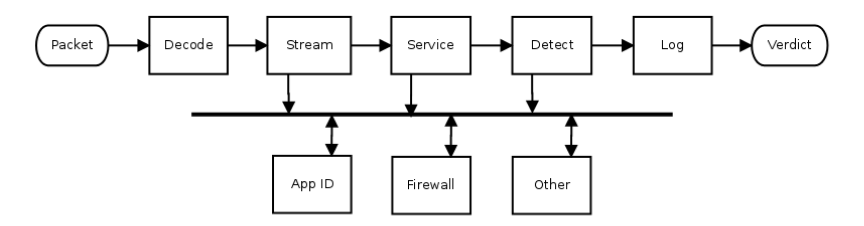
\includegraphics[width=0.8\textwidth]{resources/snort3.png}
      \caption[Arsitektur Snort versi 3]{Arsitektur Snort versi 3}
    \end{figure}
    
    Modul penangkap bertujuan mengambil paket dari lalu lintas jaringan. Lalu paket akan diproses dengan modul \emph{decoder} akan mengidentifikasi protokol paket dan mengklasifikasikannya berdasarkan spesifikasi data-link. Preproses bertujuan mengolah paket berdasarkan jenis protokol paket untuk kemudian siap dideteksi. Ini sekarang dilakukan dalam komponen \emph{service}. Preproses juga bertujuan menyusun fragmen IP dan \emph{stream} TCP yang dilakukan pada komponen \emph{stream}. Selain itu paket juga dicek jika berada diluar TCP \emph{window}, dan akan disusun ulang. 
    
    Kemudian, paket akan masuk modul pencocokan. Modul ini akan mengelompokkan \emph{rule} dan paket berdasarkan grup yang disusun berdasarkan protokol, port, dan servis. Lalu terakhir, paket akan dicek oleh modul detektor menggunakan \emph{rule} yang tersedia dan mengirimkan hasilnya ke modul keluaran.

    % \footnotetext{Snort}

  \subsection{\emph{Rule} Snort NIDPS}

  \emph{Rule} adalah kumpulan kata kunci yang digunakan dalam mendeteksi kemungkinan pelanggaran kebijakan keamanan. Snort akan melakukan pencocokan paket berdasarkan kondisi yang ditentukan dalam tiap \emph{rule}. \emph{Rule} memiliki struktur dasar berupa \emph{header} dan \emph{body} seperti pada Gambar II.2 berikut. 
  
      \begin{figure}[htb]
        \centering
        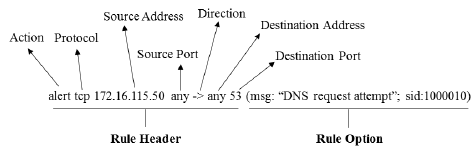
\includegraphics[width=0.8\textwidth]{resources/rule.png}
        \caption[Struktur \emph{rule} Snort NIDPS]{Struktur \emph{rule} Snort NIDPS}
      \end{figure}
  
      % \footnotetext{Snort}

    \emph{Header} berisi spesifikasi dari berupa aksi, protokol, IP sumber, port sumber, operator, IP tujuan, port tujuan. Operator menandai arah dari paket. Arah paket bisa satu atau dua arah. Aksi akan dijalankan jika signature paket cocok dengan \emph{rule} \citep{5358130}. Sedangkan \emph{body rule} berisi kumpulan \emph{option} yang digunakan untuk pencocokan paket. 

    Beberapa \emph{option} yang biasa digunakan dalam Snort \emph{Rule} diantaranya:
    \begin{enumerate} 
      \item \emph{sid}, ID \emph{rule}
      \item \emph{msg}, pesan kesalahan yang ditampilkan ke pengelola atau \emph{log}
      \item \emph{flow}, arah aliran paket dari atau ke server
      \item \emph{flags}, flag TCP yang dicari
      \item \emph{content}, konten yang dicocokkan berupa teks
      \item \emph{reference}, acuan dari \emph{vulnerability} yang mungkin
    \end{enumerate} 

% \section{Komputasi Paralel}

%   % \blindtext

%   \subsection{Hukum Amdahl dan Hukum Gustafson}

%     Secara optimal, speedup yang dicapai dengan paralelisasi akan tumbuh secara linier. Namun kenyataannya, paralesisasi terbatas dengan porsi sistem yang dapat diparalelkan. Sehingga, speedup maksimum yang akan dicapai hanya akan sebesar konstanta tertentu \citep{amdahl}. Hipotesis ini dikenal dengan Hukum Amdahl dengan persamaan

%     \begin{equation}
%       S_{latensi}(s) = \frac{1}{1 - p + \frac{p}{s}}
%     \end{equation} \\
%     dengan $Q$ adalah jumlah simpul dan $P$ adalah jumlah pola.

%     Hukum Amdahl hanya berlaku pada kasus dengan ukuran masalah yang tetap. Pada prakteknya, semakin besar kapasitas komputasi, ukuran masalah yang dipecahkan juga semakin besar dengan jumlah data yang juga besar, sehingga waktu yang dihabiskan pada porsi sistem yang dapat diparalelkan juga makin besar \citep{gustafson}. Berdasarkan fakta tersebut, Gustafson mengajukan perbaikan pada Hukum Amdahl

%     \begin{equation}
%       S_{latensi}(s) = 1 - p + sp
%     \end{equation} \\

%     Terlihat bahwa Hukum Gustafson membuat speedup maksimum menjadi lebih linier dan realistis.

%   \subsection{\emph{Multiprocessing} dan \emph{Multithreading}}

%     Proses adalah program yang sedang dieksekusi. Ketika proses dijalankan, dia memiliki beberapa status: baru, berjalan, menunggu, siap, dan berhenti. Tiap proses memiliki informasi mengenai alokasi memori, status proses, dan isi CPU register yang disebut dengan konteks \citep{os}. Ketika proses ini pertama dilanjutkan dari keadaan menunggu, maka CPU akan memuat konteks proses. Jika ada, proses lain yang akan berjalan, maka CPU akan mengganti konteks proses dengan konteks proses baru yang akan berjalan. Hal ini dikenal dengan \emph{context switching}.

%     Satu proses dapat memiliki banyak thread. Thread didefinisikan sebagai unit terkecil eksekusi dari CPU \citep{os}. Thread dikenal pula dengan proses ringan. Berbeda dengan proses, thread pada proses yang sama dapat berbagi memori yang sama. Penggunaan thread dapat memungkinkan operasi yang IO-bound dan CPU-bound dapat berjalan bersamaan.

%     Multiprocessing yaitu teknik untuk menggunakan proses yang berbeda untuk melakukan suatu pekerjaan. Sedangkan multithreading yaitu teknik yang memungkinkan satu unit pemroses (seperti CPU dan GPU) untuk mengeksekusi banyak thread secara konkuren. Keuntungan multithreading dibandingkan multiprocess adalah masing-masing thread akan berbagi resource dari unit komputasi, seperti memori, cache dan translation lookaside buffer (TLB). Selain itu, komunikasi antar thread juga bisa dilakukan dengan menggunakan memori bersama. 

%   \subsection{Sinkronisasi}

%     Multithreading memungkinkan kita untuk saling berbagi memori yang sama. Namun, ada kerugian dari adanya sharing resource ini. Task antar thread harus menjamin bahwa mereka tidak mengakses dan menimpa memori yang sama atau mereka akan mengakibatkan nilai memori menjadi tidak konsisten. Masalah ini dikenal dengan \emph{race condition}. Race condition terjadi ketika dua atau lebih thread memasuki wilayah yang seharusnya hanya boleh dimasuki satu thread yang disebut \emph{critical section}. 

%     Untuk menghindari terjadinya race condition kita dapat melakukan sinkronisasi proses. Ada beberapa metode sinkronisasi proses yang akan digunakan pada penelitian ini:

%     \begin{enumerate}

%     \item
%     Mutex lock \\
%     Mutex 

%     \item
%     Semaphore \\

%     \item
%     Barrier \\

%     \end{enumerate}

%  Ketika beberapa thread akan menggunakan critical section, maka flag akan dipasang untuk mencegah thread lain masuk dalam critical section tersebut. Ketika thread tersebut telah keluar dari critical section, flag akan dicabut kembali dan thread lain akan dapat masuk ke dalam critical section. 

%     Ada banyak jenis implementasi dari flag yang 
%Hal ini bisa diatasi dengan memasang lock pada resoure yang mungkin akan diakses bersama-sama. Lock dapat memandaatkan mutex lock, semaphore, atau dll.

% \section{Struktur Data Trie}

  %Struktur data \emph{trie} adalah struktur data yang digunakan untuk menyimpan himpunan dinamis dari beberapa string \citep{trie59}. Struktur data trie merupakan jenis dari struktur pohon yang memiliki jumlah simpul anak yang tidak tentu. 
  % Secara umum, \emph{trie} dapat menggambarkan dengan .  % 
  %Simpul akar \emph{trie} akan dimulai dari simpul kosong. Lalu bercabang ketika ada karakter yang berbeda. Sehingga pencarian string dalam kamus dapat dilakukan dengan menelusuri tiap simpul pada \emph{trie}. Trie dapat dimodelkan sebagai sebuah finite automata. Tiap simpul dapat dimodelkan sebagai status dan huruf atau substring dimodelkan sebagai fungsi transisi. Lalu, setiap simpul awal dan simpul akhir akan ditandai secara khusus. Ketika simpul akhir tercapai, berarti salah satu pola ditemukan.

  %\begin{figure}[htb]
  %    \centering
  %    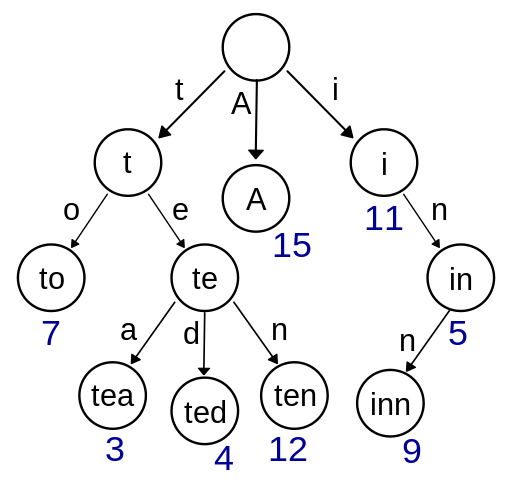
\includegraphics[width=0.8\textwidth]{resources/trie.png}
  %    \caption[Contoh trie untuk kata "A","to", "tea", "ted", "ten", "i", "in", dan "inn"]{Contoh trie untuk kata "A","to", "tea", "ted", "ten", "i", "in", dan "inn"}
  %  \end{figure}

  %Strategi implementasi yang biasa dilakukan yaitu dengan menggunakan list untuk menyimpan simpul anak sebanyak jumlah karakter maksimal pada tiap simpul. Bisa juga menggunakan tabel statik untuk menyimpan referensi ke simpul anak. 

  %\subsection{Bitwise Trie}

  %  Bitwise Trie adalah varian trie yang menggunakan operasi bit untuk penelusuran simpul. Berbeda dari trie yang menggunakan karakter sebagai fungsi transisi, bitwise trie hanya memiliki dua simpul anak tiap simpulnya. Meski terlihat lambat, metode ini mengoptimalkan cache lokal

  %\subsection{Trie dengan Kompresi}

\section{\emph{Pattern Matching}}

  \emph{Pattern matching} adalah metode mencari kemunculan sebuah string atau substring terhadap string lain. \emph{Pattern matching} menjadi salah satu komponen inti dalam NIDPS. Secara umum ada dua jenis utama pencocokan pola, yaitu \emph{single pattern matching} dan \emph{multi-pattern matching}. 
  
  \emph{Single pattern matching} yaitu pencocokan masukan terhadap satu pola. Algoritma yang tergolong \emph{single pattern matching} yaitu algoritma Knuth-Morris-Pratt dan Boyer-Moore. Sementara itu, \emph{multi-pattern matching} mencocokkan masukan terhadap beberapa pola sekaligus. Algoritma yang termasuk dalam \emph{multi-pattern matching} yaitu algoritma Aho-Corasick dan Wu-Manber, yang merupakan modifikasi dari algoritma Boyer-Moore. 
  
  Masalah yang akan diselesaikan dalam pencocokan pola pada IDS merupakan \emph{multipattern string matching}. Algoritma Wu-Manber tidak digunakan dalam implementasi Snort versi 3.0. Sehingga fokus eksperimen ini yaitu algoritma Aho-Corasick.


  \subsection{Algoritma Aho-Corasick}

    Algoritma Aho-Corasick adalah algoritma \emph{multi-pattern matching} yang dapat mencari kemunculan string dalam sebuah kamus \citep{ahoc1975}. Algoritma ini dapat mencari kemunculan setiap string dalam kamus dalam sekali pencocokan. Komponen utama dalam algoritma ini yaitu kamus yang berupa \emph{finite automata} seperti pada Gambar II.3 di bawah. %dan \emph{failure transition}.

    Kamus berisi kumpulan string \emph{rule} yang akan dicocokkan. Penyusunan kamus hanya perlu dilakukan sekali sebelum pencocokan string dilakukan. Penyusunan kamus dilakukan dalam $O(kp)$, dengan $k$ adalah jumlah string pada kamus dan $p$ adalah panjang maksimum string pada kamus.

    \begin{figure}[htb]
      \centering
      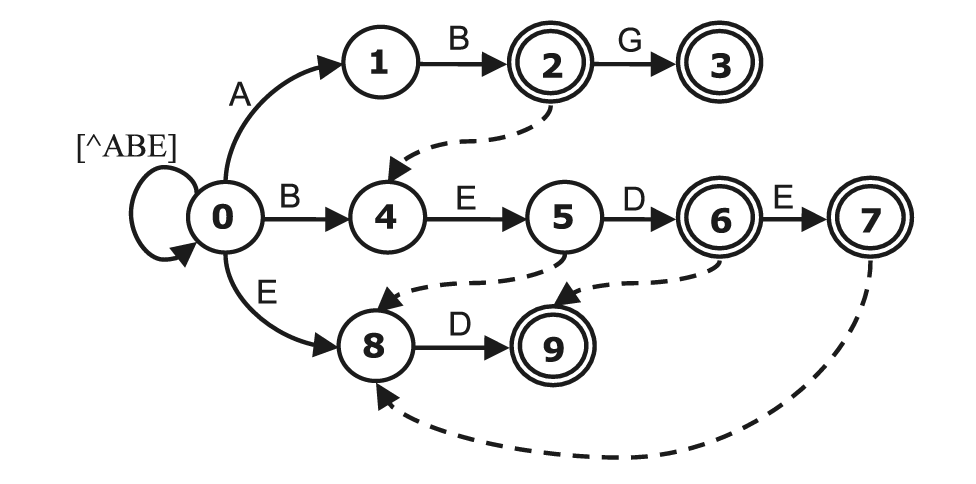
\includegraphics[width=0.6\textwidth]{resources/aho-c.png}
      \caption[\emph{Finite automata} kamus algoritma Aho-Corasick dengan \emph{failure transition}]{\emph{Finite automata} kamus algoritma Aho-Corasick dengan \emph{failure transition} \citep{lin2013}}
    \end{figure}

    % \footnotetext{\citep{lin2013}}

    Dalam kamus ada yang disebut \emph{failure transition}. \emph{Failure transition} adalah tabel yang berisi posisi terakhir prefiks yang cocok dengan sufiks string yang telah dilewati. Sehingga ketika pencarian tidak cocok pada suatu string, akan dilanjutkan pada string berikutnya yang prefiksnya cocok dengan sufiks string sebelumnya. Tujuan adanya \emph{failure transition} yaitu untuk menghindari pengulangan ketika adanya \emph{mismatch}. Kompleksitas pencarian algoritma ini yaitu $O(x)$, dengan $x$ adalah panjang string pola.

  \subsection {Pembentukan Kamus}

    Kamus dalam Aho-Corasick dibentuk dari kumpulan \emph{string} masukan. Pembentukan kamus dimulai dari \emph{state} awal yang berupa \emph{string} kosong. Kemudian tiap \emph{string} akan ditelusuri per huruf. Tiap huruf akan menjadi transisi ke \emph{state} baru. Ketika penelusuran telah mencapai akhir \emph{string}, maka \emph{state} ditandai sebagai \emph{state} akhir.

    Langkah selanjutnya yaitu membentuk \emph{failure function}. \emph{Failure function} dari tiap \emph{state} adalah prefiks terpanjang pada kamus yang sama dengan sufiks pola. Transisi \emph{failure function} dicari dengan melakukan iterasi pada \emph{previous state}. Tiap \emph{previous state} akan dicek apakah ada \emph{failure function} yang memiliki transisi yang sama dengan \emph{state} yang ingin dibentuk \emph{failure function}-nya. Ketika ada prefiks yang lebih panjang, maka \emph{failure function} akan diperbarui.
    
  \subsection {\emph{Boundary Detection Problem}}
    
    Untuk dapat meningkatkan kinerja algoritma Aho-Corasick, string dapat dipartisi menjadi beberapa segmen. Sehingga tiap partisi dapat dicocokkan menggunakan satu \emph{thread}. Namun terdapat ada masalah pada pencocokan partisi ketika pola yang dicari ternyata berada pada lebih dari satu partisi. Bagian pola akan terpotong seperti pada Gambar II.4 di bawah dan tidak dapat dideteksi. Masalah ini dikenal sebagai \emph{boundary detection problem}. 
    
    \begin{figure}[htb]
      \centering
      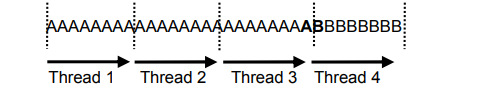
\includegraphics[width=0.5\textwidth]{resources/boundary.png}
      \caption[\emph{Boundary detection problem} terjadi pada pola "AB" tidak terbaca oleh \emph{thread} 3 dan 4]{\emph{Boundary detection problem} terjadi pada pola "AB" tidak terbaca oleh \emph{thread} 3 dan 4 \citep{lin2013}}
    \end{figure}
    
    Solusi dari masalah itu yaitu dengan menambah jangkauan pencocokan sepanjang $m - 1$, yaitu panjang pola terpanjang dikurangi satu. Total kompleksitas yang diperoleh tiap thread menjadi $O(n/s + m)$ dengan $n$ adalah panjang masukan dan $s$ adalah banyak segmen yang dibentuk. Sehingga total kompleksitas untuk \emph{lookup} memori menjadi $O((n/s + m) * s) = O(n + ms)$. Dibandingkan dengan \emph{lookup} pada Aho-Corasick biasa yang hanya $O(n)$, operasi ini dapat menjadi bottleneck pada pencarian pola.
    
    % \footnotetext{\citep{lin2013}}

  \subsection {\emph{Parallel Failureless Aho-Corasick}}

    Algoritma \emph{Parallel Failureless Aho-Corasick} (PFAC) merupakan pengembangan dari algoritma Aho-Corasick untuk melakukan pencocokan dengan \emph{multithreading}. PFAC menggunakan \emph{state machine} yang tidak mengandung \emph{failure transition} dan masing-masing \emph{thread} memulai pencocokan dari tiap satu karakter masukan \citep{lin2013}. Bentuk \emph{state machine} PFAC terlihat seperti pada Gambar II.5.

    \begin{figure}[htb]
      \centering
      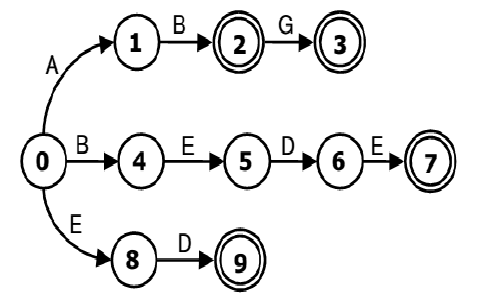
\includegraphics[width=0.5\textwidth]{resources/pfac.png}
      \caption[\emph{Finite automata} Aho-Corasick tanpa \emph{failure transition}]{\emph{Finite automata} Aho-Corasick tanpa \emph{failure transition} \citep{lin2013}}
    \end{figure}
    
\section{\emph{General-Purpose computing on Graphics Processing Units}}
  
  \emph{General-purpose computing on graphics processing units} (GPGPU, kadang disebut juga GPGP atau GP\textsuperscript{2}U) adalah teknik untuk menggunakan pemroses grafis / GPU untuk melakukan komputasi umum yang biasa dilakukan pada pemroses CPU. Teknik ini memanfaatkan desain GPU berbeda dari CPU yang khusus digunakan untuk memroses grafik dengan unit piksel yang sangat banyak. Sehingga GPU memiliki banyak \emph{core} yang berjalan paralel dan berbeda dari CPU yang biasa digunakan untuk melakukan operasi sekuensial \citep{lindholm2001}. Dalam GPU terdapat beberapa \emph{stream multiprocessor} (SM) yang masing-masing memiliki beberapa \emph{core thread} atau \emph{stream processor} (SP). Ilustrasi perbedaan CPU dan GPU terlihat seperti pada Gambar II.6 berikut.

  % \footnotetext{\citep{lin2013}}
    
  \begin{figure}[htb]
    \centering
    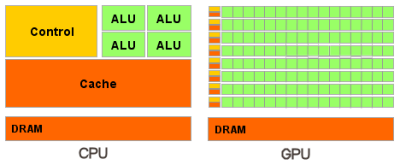
\includegraphics[width=0.8\textwidth]{resources/GPUvsCPU.png}
    \caption[Perbedaan arsitektur CPU dan GPU]{Perbedaan arsitektur CPU dan GPU \citep{cuda}}
  \end{figure}
    
  % \footnotetext{Cuda}

  \subsection{Struktur Memori}
    
    Tiap \emph{core thread} memiliki memori lokal yang saling independen. Dalam tiap blok, \emph{thread} yang ada dalam blok dapat mengakses \emph{shared memory}. Kemudian ada memori global yang dapat diakses semua \emph{thread}. Hirarki memori GPU kurang lebih seperti pada Gambar II.7.
    
    Ada perbedaan kecepatan ketika melakukan operasi pada tiap tingkatan memori. Makin tinggi tingkatan memori, makin besar latensi akses memori. Urutan besar latensi akses memori yaitu memori lokal, memori bersama, kemudian memori global. Sehingga diutamakan menggunakan memori yang lebih rendah dahulu. Jika membutuhkan sinkronisasi antar \emph{thread}, memori yang lebih tinggi dapat digunakan. 
    
    \begin{figure}[htb]
      \centering
      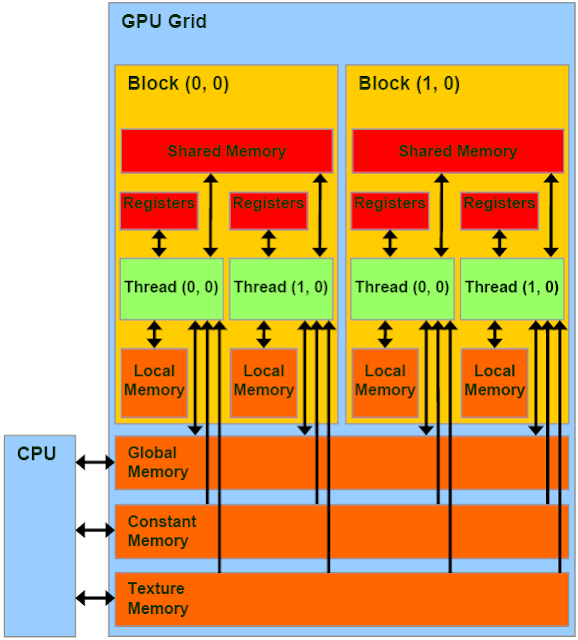
\includegraphics[width=0.6\textwidth]{resources/cudamem.png}
      \caption[Tingkatan memori GPU]{Tingkatan memori GPU \citep{cuda}}
    \end{figure}

    % \footnotetext{Nvidia}

    Selain ketiga memori tersebut, ada juga memori yang hanya dapat ditulis oleh \emph{host} yaitu memori konstanta dan tekstur. Kedua memori ini hanya dapat ditulis sekali sebelum \emph{kernel} dipanggil. Keuntungan menggunakan kedua memori ini yaitu latensi akses yang lebih kecil dari memori global. Hal ini terjadi karena kedua memori ini memanfaatkan \emph{locality} dalam akses memori. Memori konstanta menggunakan \emph{cache} sehingga akses untuk memori yang sama berkali-kali akan sangat cepat. Sedangkan memory tekstur menggunakan \emph{spatial locality} untuk \emph{thread} yang berdekatan.

  % Saat ini ada dua platform GPGPU yang populer, CUDA dan OpenCL. CUDA adalah platform yang dikembangkan oleh NVIDIA. CUDA hanya dapat berjalan pada perangkat milik NVIDIA. Sedangkan OpenCL dikembangkan oleh grup konsorsium Khronos. OpenCL dapat berjalan pada banyak perangkat, seperti CPU, GPU, FPGA, dan DSP (\emph{digital signal processor})).
  
  %Penelitian tentang GPGPU dimulai ketika \emph{programmable pixel} dan \emph{vertex shaders} diperkenalkan. Penggunaan GPGPU lebih mudah dengan adanya \emph{shading language} yang berjalan pada GPU. \emph{Shading language} adalah bahasa pemrograman yang spesifik untuk mendeskripsikan tampilan sebuah \emph{scene} \citep{proudfoot2001}. \emph{Shading language} bertujuan menyediakan antarmuka \emph{high level} untuk operasi \emph{vertex} pada GPU. 
  
  %Dengan adanya \emph{shading language}, operasi vektor dan matriks dapat dengan mudah diubah menjadi operasi \emph{vertex}. Sejak saat itu, usaha untuk melakukan komputasi umum dengan GPU mulai bermunculan seperti perkalian matriks \citep{matrix2001}, simulasi fisika \citep{phys2002}, hingga dekomposisi LU pada matriks persegi \citep{lugpu2005}. Maka, pada tahun 2003, dalam disertasinya \citep{harris2003}, Mark Harris mengajukan sebuah istilah yang kini dikenal sebagai \emph{general-purpose computing on graphics processing units} (GPGPU) sekaligus mendirikan situs GPGPU.org.
  
  \subsection{\emph{Compute Unified Device Architecture}}
  
    \emph{Compute Unified Device Architecture} (CUDA) adalah platform dan API untuk GPGPU oleh NVIDIA. CUDA menyediakan antarmuka untuk dapat menggunakan GPU NVIDIA untuk melakukan GPGPU \citep{cuda}. CUDA API dapat diimplementasi menggunakan bahasa C, C++, dan Fortran. Selain itu, ada juga \emph{binding} yang dibuat dalam pustaka beberapa bahasa oleh pihak ketiga, seperti Python, Perl, Java, Ruby, Haskell, Lua, MATLAB, dan Mathematica.
    
    \subsubsection{Struktur Kode CUDA}
    
      Terdapat dua perangkat yang berbeda untuk \emph{runtime} CUDA, yaitu \emph{host} (CPU), dan \emph{device} (GPU). Masing-masing platform akan menjalankan bagian kode tersendiri. Ada dua bagian dalam kode program CUDA, yaitu \emph{host code} dan \emph{kernel code}. Ketika program berjalan, maka \emph{host code} akan berjalan terlebih dahulu. Lalu, \emph{kernel code} akan disalin dan dijalankan di memori GPU. Karena memori yang dapat diakses oleh masing-masing kode juga terpisah, maka perlu dilakukan alokasi pada memori \emph{device} dan transfer antar memori \emph{device} dan memori \emph{host}.
    
    \subsubsection{CUDA \emph{Thread}}
    
      CUDA \emph{thread} dibagi menjadi beberapa kelompok blok yang disebut \emph{grid}. Masing-masing \emph{grid} berisi beberapa buah blok. Di dalam blok terdapat beberapa \emph{thread} yang akan berjalan terpisah. Struktur \emph{thread} CUDA kurang lebih seperti pada Gambar II.8.
      
      \begin{figure}[htb]
        \centering
        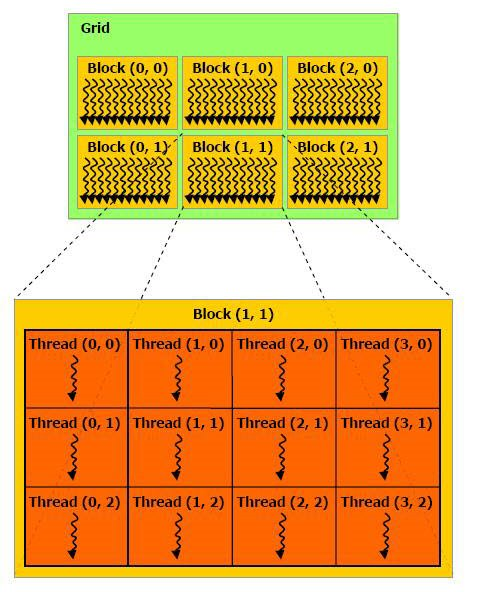
\includegraphics[width=0.8\textwidth]{resources/cudathread.jpg}
        \caption[Organisasi \emph{thread} CUDA]{Organisasi \emph{thread} CUDA \citep{cuda}}
      \end{figure}
      
      CUDA \emph{thread} memiliki indeks, yang berdimensi 3. Indeks \emph{thread} akan menunjukkan nomor blok dan nomor \emph{thread} tersebut dalam blok. Menggunakan kedua indeks tersebut, dapat dibentuk nomor yang unik tiap \emph{thread}. Nomor unik tersebut dapat digunakan untuk melakukan pemrosesan paralel pada data besar. Hingga CUDA versi 8.0, maksimum dimensi blok \emph{thread}, dimensi grid, dan jumlah \emph{thread} tiap blok berturut-turut adalah 1024 x 1024 x 64, 65535 x 65535 x 65535, dan 1024.

      % \footnotetext{\citep{cuda}}

    \subsubsection{\emph{Warp} dan Percabangan}

      \emph{Thread} akan dieksekusi bersama-sama dalam sebuah kumpulan yang disebut \emph{warp}. \emph{Thread} yang berjalan dalam satu \emph{warp} akan mengeksekusi instruksi yang sama dalam satu waktu. Ketika ada percabangan dalam instruksi, maka \emph{warp} tersebut akan berpisah. Ukuran maksimal \emph{warp} saat ini yaitu 32 \emph{thread}.

      Karena percabangan mempengaruhi eksekusi \emph{warp}, maka penempatan kondisi harus dilakukan secara hati-hati. Jika percabangan tidak dilakukan dengan benar dan menyebabkan banyak \emph{thread} terpisah, maka akan banyak \emph{warp} yang akan terbuang karena hanya mengeksekusi sedikit \emph{thread}.
      
      Pada GPU arsitektur Fermi, terdapat fitur yang disebut \emph{memory coalescing}. \emph{Memory coalescing} terjadi ketika semua \emph{thread} pada \emph{warp} yang sama mengakses memori yang kontigu. Fitur ini memungkinkan akses memori yang kontigu tersebut dilakukan dalam sekali \emph{request}.

\section{Penelitian Terkait}

  \subsection{Rancangan \emph{Multithreading} pada Pencocokan NIDS Berbasis \emph{Signature}} 

    Penelitian terkait optimasi berbasis \emph{multithreading} pada NIDS telah dilakukan oleh \cite{multi2004}. Tujuan optimasi yaitu untuk meningkatkan kapasitas pencocokan \emph{signature}. Optimasi dilakukan berdasarkan pada beberapa strategi berikut:

    \begin{enumerate}
      \item \emph{Thread asynchronous} untuk modul keluaran
      \item Pencocokan \emph{signature} secara \emph{multithread}
      \item Normalisasi konteks dan pencocokan \emph{signature} secara \emph{multithread}
      \item Pencegahan \emph{stateful}, normalisasi konteks dan pencocokan \emph{signature} secara \emph{multithread}
      \item Pencegahan \emph{stateful} secara \emph{multithread} dengan normalisasi konteks dan pencocokan \emph{signature} secara \emph{multithread} terpisah
    \end{enumerate}

    Hasil yang diperoleh dengan pengukuran pada prosesor Intel Xeon dengan \emph{hyper-threading} menunjukkan bahwa desain 2 dan 3 memiliki kinerja yang rata-rata lebih baik dari pada desain lainnya. Pada desain 2 diperoleh penurunan \emph{runtime} menjadi 94,1\% dan 86,1\%, untuk menggunakan \emph{hyper-threading enabled} dan tidak. Sedangkan pada desain 3, diperoleh \emph{runtime} 89\% dan 84\%. Sementara itu pada desain 4 dan 5 malah terjadi peningkatan \emph{runtime} sebesar 120\% hingga 150\%. Hal ini disebabkan \emph{latency} dari penggunaan struktur data yang rumit dan memerlukan banyak sinkronisasi.

  \subsection{Rancangan NIDS berbasis GPGPU}

    Selain rancangan \emph{multithreading} pada CPU, telah dilakukan penelitian tentang rancangan arsitektur untuk NIDS pada GPGPU oleh \cite{gnort2008}. Rancangan bertujuan mengakomodasi implementasi algoritma Aho-Corasick pada GPU. Implementasi berdasarkan pada NIDS Snort. Beberapa komponen yang dimodifikasi yaitu implementasi \emph{state machine} dan skema transfer antara \emph{host} dan \emph{device}. 

    Implementasi menggunakan struktur memori untuk menyimpan pola \emph{signature} yang berbentuk \emph{list of string}. \emph{Layout} ini kemudian dimodfikasi menjadi \emph{array} 2D sebelum diimplementasi menggunakan CUDA. Kelebihan \emph{layout} memori ini adalah mudah untuk ditransfer ke memori tekstur. Selain itu algoritma Aho-Corasick memanfaatkan prinsip \emph{locality} dengan baik. Sehingga implementasi memori dapat meningkatkan kinerja pencocokan NIPS hingga 19\%.

    Transfer data dari \emph{host} ke \emph{device} maupun \emph{device} ke \emph{host} menggunakan skema \emph{double buffering}. Skema ini menggunakan sebuah \emph{buffer} untuk menampung paket yang ingin dicek menjadi satu batch besar. Batch besar kemudian ditransfer ke memori \emph{device}. Ketika GPU melakukan pemrosesan, maka paket yang baru datang akan ditampung dalam \emph{buffer} berbeda. Sehingga kedua \emph{buffer} dapat selalu bertukar posisi. Hal ini mampu meningkatkan utilitas pengiriman rata-rata paket. 
    
    Selain itu, memori \emph{host} dapat dikonfigurasi menggunakan \emph{pinned memory}. Penggunaan \emph{pinned memory} membuat penempatan memori menjadi statik sehingga mengurangi tingkat \emph{memory page swapping} dan juga meningkatkan \emph{throughput} keseluruhan sistem.

    Ada 2 desain pencocokan paket yang diteliti:
    \begin{enumerate}

      \item Pencocokan paralel paket tunggal \\
      Paket akan dibagi menjadi fragmen-fragmen dan disebar merata pada tiap \emph{thread}. Kelebihan dari skema ini yaitu masing-masing \emph{thread} mendapat bagian yang setara dan waktu yang diperlukan untuk pencocokan relatif sama sehingga tidak perlu saling menunggu. Sedangkan kekurangan dari skema ini adalah pencocokan akan mengalami \emph{overlap} satu sama lain dan perlu penanganan khusus.

      \item Pencocokan paralel multipaket \\
      Masing-masing paket akan didelegasikan pada satu \emph{thread} pada \emph{stream processor}. Kelebihan dari skema ini adalah pencocokan tidak akan mengalami \emph{overlap}. Sedangkan kekurangan dari skema ini adalah masing-masing \emph{thread} sering menunggu satu sama lain karena ukuran paket yang berbeda-beda.

    \end{enumerate}

    Berdasarkan pengujian yang menggunakan 1000 pola acak, pencocokan dengan GPU mendapat \emph{throughput} hingga 2,3 Gbps untuk paket rata-rata sebesar 1500 \emph{byte}. Peningkatan yang berhasil dicapai sebesar 3,2 kali lipat dari \emph{multithread} CPU. Spesifikasi lingkungan pengujian yaitu GPU NVIDIA GeForce 8600GT 1,2 GHz dengan 32 \emph{stream processor} dalam 4 \emph{stream multiprocessor} dengan memori 512 MB, dan CPU Intel Pentium 4 3,4 Ghz dengan memori 2 GB.

  \subsection{Rancangan Algoritma Pencocokan \emph{Multiple-pattern} pada NIDS Berbasis GPU}

    \cite{4482891} mengajukan implementasi algoritma turunan Wu-Manber agar dapat memanfaatkan paralelitas pada GPU. Implementasi dilakukan dengan \emph{shading language} yaitu Cg. Pencocokan akan memanfaatkan \emph{fragment processor}. \emph{Fragment processor} adalah pemroses yang bertugas melakukan operasi pemetaan tekstur terhadap fragmen masukan dan menuliskan hasilnya ke \emph{rendering} target yang berupa \emph{framebuffer} atau memori tekstur.

    Tabel pola dan paket masukan disimpan pada memori tekstur. Penyimpanan dapat berupa tabel dua atau tiga dimensi. Selain pola dan paket, informasi tentang \emph{prefilter} dan paket kandidat juga disimpan di memori tekstur dalam bentuk \emph{hash}. \emph{Hash} berfungsi menggantikan \emph{shift-byte table} pada algoritma Wu-Manber untuk lompat ke pola terdekat dan melewati karakter yang tidak perlu.

    Hasil yang diperoleh yaitu peningkatan \emph{throughput} hingga 3 kali dibandingkan implementasi Wu-Manber pada Snort. Struktur tekstur yang digunakan sangat berpengaruh terhadap latensi. Implementasi dengan representasi larik satu dimensi lebih cepat 1,5 kali lipat dibandingkan representasi tabel. Hal ini disebabkan struktur 2D memiliki banyak \emph{branching overhead} karena \emph{hash collision}.

  \subsection{Rancangan NIDS Berbasis \emph{Signature} yang \emph{Scalable} pada GPU}

    Dalam penelitiannya, dijelaskan oleh \cite{kargus2012} bahwa pada NIDPS, \emph{bottleneck} utama terdapat pada 3 komponen, \emph{packet acquisition}, \emph{multi-string pattern matching}, dan pencocokan opsi \emph{rule}. Pencocokan opsi \emph{rule} hanya dilakukan saat paket terindikasi mengandung serangan oleh tahap \emph{multistring pattern matching}. 
    
    Opsi dapat mengandung PCRE (\emph{Perl Compatible Regular Expression}). Sebelum PCRE dicocokkan, PCRE akan dipreproses menjadi DFA terlebih dahulu menggunakan algoritma Thompson. Kemudian pencocokan opsi dapat dilakukan menggunakan metode yang serupa dengan pencocokan \emph{multistring}.

    Sehingga dalam penelitian ini, diajukan beberapa optimasi untuk pencocokan \emph{rule option}. Salah satu optimasi yang diajukan untuk tahap pencocokan yaitu penggunaan \emph{pipelining}. \emph{Pipelining} dilakukan dengan memisahkan \emph{thread} yang digunakan untuk operasi \emph{I/O} dengan operasi analisis. Kemudian pada tiap operasi \emph{I/O}, akan dilakukan pengumpulan paket dalam \emph{batch} sebelum dilakukan transfer antar komponen. Implementasi dilakukan dengan menggunakan basis IDS Snort.

    Pengujian dilakukan dengan konfigurasi CPU ganda Intel X5680 dengan 12 core dan dua GPU NVIDIA GTX 580. Hasil yang didapatkan menggunakan desain ini mampu mencapai 1,5 sampai 4 kali lipat kinerja Snort. \emph{Latency} dapat menurun hingga 13 mikrodetik pada \emph{offloading} paket awal untuk batch sebesar 1,5 kB. Pada pengujian dengan \emph{traffic} jaringan, rancangan ini mampu mencapai \emph{throughput} 25,2 Gbps pada \emph{input} sebesar 40 Gbps.

  \subsection{Optimasi Algoritma Pencocokan Pola pada GPU}

    Salah-satu algoritma yang sering digunakan dalam deteksi pola adalah Aho-Corasick yang bersifat \emph{multi-pattern string matching}. Dalam penelitian yang dilakukan \cite{lin2013}, dilakukan optimasi pada implementasi algoritma Aho-Corasick pada GPU. Implementasi memanfaatkan fitur-fitur pada GPU seperti \emph{memory coalescing}, penghematan transaksi pada \emph{global memory}, dan akses \emph{shared memory} yang bebas \emph{bank-conflict}.

    Desain akan menggunakan pendekatan algoritma AC tanpa \emph{failure function} yaitu PFAC (\emph{Parallel Failureless Aho-Corasick}). Pendekatan ini dapat memaksimalkan penggunaan \emph{thread} pada GPU tanpa menyebabkan \emph{overlapping}. Transaksi ke \emph{global memory} dapat dikurangi dengan memuat transisi \emph{state} kosong ke \emph{shared memory} dan penggunaan \emph{texture memory} yang memanfaatkan \emph{cache}.

    Hasil pengujian dengan CPU Intel Core i7-950 dan GPU NVIDIA GTX 580 menunjukkan peningkatan yang signifikan. Optimasi dengan PFAC pada \emph{multithread} CPU mencapai 7 kali lipat dari AC. Sedangkan PFAC pada GPU dapat mencapai 10 kali lipat daripada AC pada CPU. Masukan didapatkan dari dataset \emph{traffic} kompetisi DEFCON.

  \subsection{Penyimpanan \emph{Signature} dengan Struktur \emph{Trie} Terkompresi}

    Penyimpanan \emph{signature} untuk NIDS dapat dilakukan dengan struktur \emph{trie} terkompresi. Desain utama \emph{trie} menggunakan representasi penelusuran \emph{breadth first search} (BFS). Lokasi \emph{pointer} simpul anak akan dihitung menggunakan \emph{sparse matrix}. Selain itu dilakukan kompresi terhadap bentuk \emph{trie} sehingga memori yang dibutuhkan lebih padat \citep{bellekens2014}.

    \emph{Sparse matrix} adalah matriks yang berisi \emph{offset} dari lokasi simpul anak terkecil dan \emph{bitmap} yang berisi flag dari semua simpul anak dalam 256 karakter ASCII. Ketika ingin melakukan penelusuran, simpul akan melakukan penghitungan karakter berdasarkan offset pertama simpul ditambah dengan kumulatif dari tiap bit. Hasil yang diperoleh adalah indeks dari simpul anak berikutnya.

    Optimasi berikutnya yaitu kompresi pada sufiks kalimat. Kompresi dilakukan dalam dua tahap: penggabungan pada huruf terakhir dan tiga huruf terakhir yang sama. Huruf terakhir dapat digabungkan karena simpul tersebut tidak memiliki anak lagi. Dan tiap simpul tersebut pasti akan menuju ke penanda akhir string. Lalu untuk tahap kedua, akan dihitung sufiks dari pola. Tiap sufiks pada tiga karakter terakhir yang sama akan digabungkan.
    
    % Jumlah simpul dapat dihitung ulang dengan persamaan berikut: \\
    % \begin{equation}
    %   Q_{final} = Q - \left(\left|P\right| - 1 \right)
    % \end{equation} \\
    % dengan $Q$ adalah jumlah simpul dan $P$ adalah jumlah pola.

    %  Jumlah kombinasi dari susunan dua karakter dapat dihitung dengan \\
    % \begin{equation}
    %   r = S^2
    % \end{equation} \\
    % dengan $r$ adalah jumlah kombinasi susunan dan $S$ adalah banyak huruf yang ada dalam string pola.

    % Maka, jumlah kombinasi dari \emph{trie} dapat diestimasi dengan \\
    % \begin{equation}
    %   \overline{L} = 
    %     \sum_{i=1}^{r} P\left(g = i \right) \cdot 2i =
    %       \sum_{i=1}^{min\left({r,n} \right)} \frac{\binom{r}{i} \binom{n - i}{i}}{\binom{n}{r}} \cdot 2i
    % \end{equation} \\
    % dengan $L$ adalah rata-rata panjang \emph{trie} setelah kompresi, $P$ adalah kemungkinan \emph{trie} memiliki sufiks unik sejumlah $i$.
